\subsubsection{Selection of Bitrates}
Video Multi-Method Assessment Fusion (VMAF) is a full reference metric for estimating human perception of video quality \cite{lin2014:fvqa}.

To estimate relevant HEVC bitrates for our source content we sample the VMAF scores for different resolutions. The reference sequences are resampled to a fixed 50 frames per seconds to avoid frame rate differences, while the distorted sequences are downsampled, encoded with CBR rate control and upsampled to 4k again using lanczos resampling. The resulting VMAF scores show an overlap between different resolutions as seen in Fig. \ref{fig:vmaf:bitrates} and the final encoding bitrates are chosen near those intersections.

\begin{figure}[h]
	\centering
	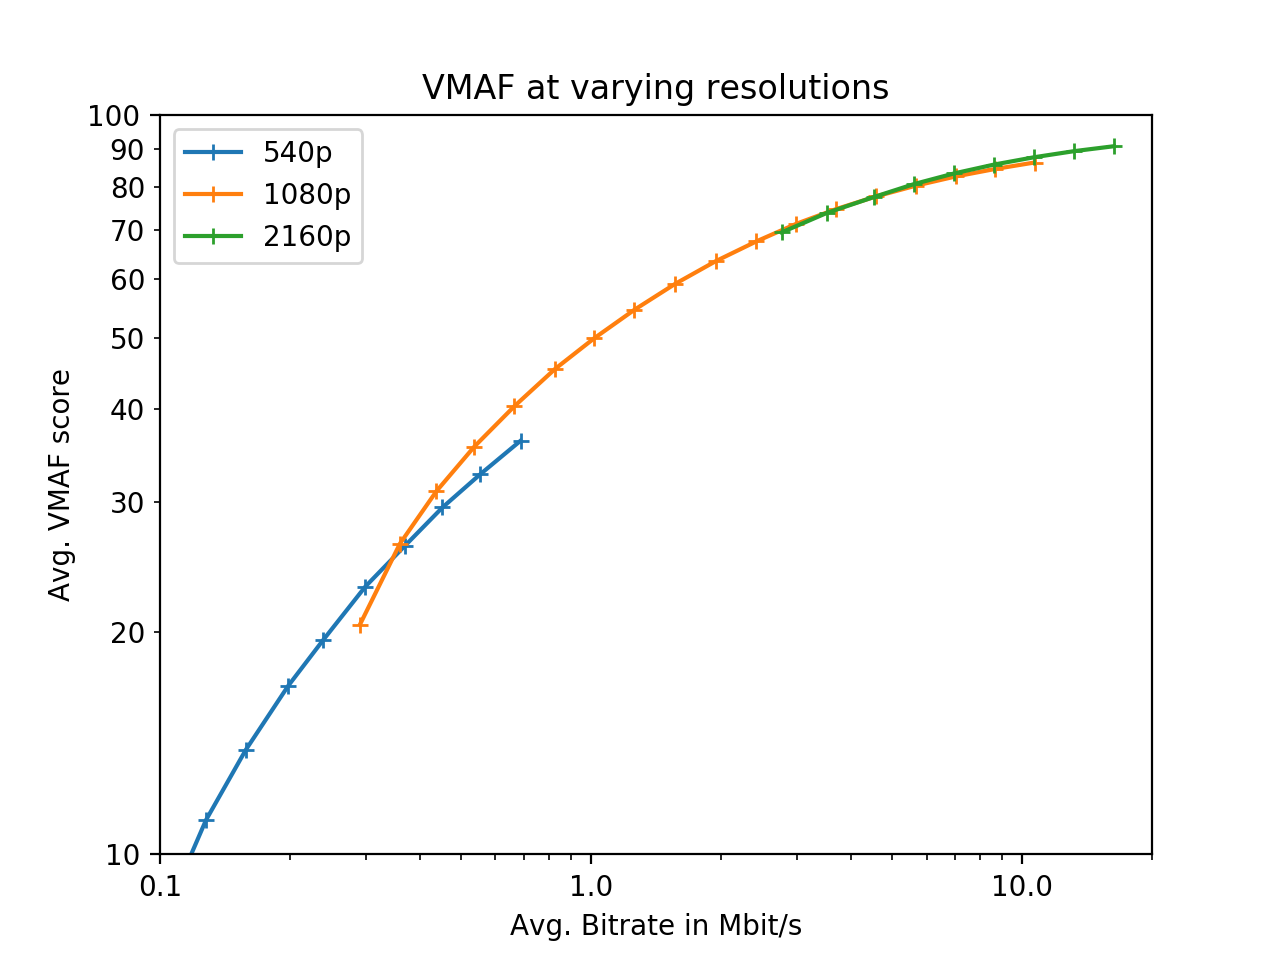
\includegraphics[width=3.5in]{vmaf_bitrates}
	\caption{VMAF scores for 25 different bitrates at 3 resolutions}
	\label{fig:vmaf:bitrates}
\end{figure}

\subsubsection{Encoding Presets}
Two different presets are used for the sequence encodings. The first is a simple CBR-encoding and the second a 2-pass encoding with a Q-CTRL pass followed by a B-CTRL pass. Every sequence is encoded with both presets at the 3 resolutions and 3 bitrates. The resulting VMAF-scores for the encoded sequences can be seen in figure \ref{fig:vmaf:encoded}.


\begin{figure}[h]
	\centering
	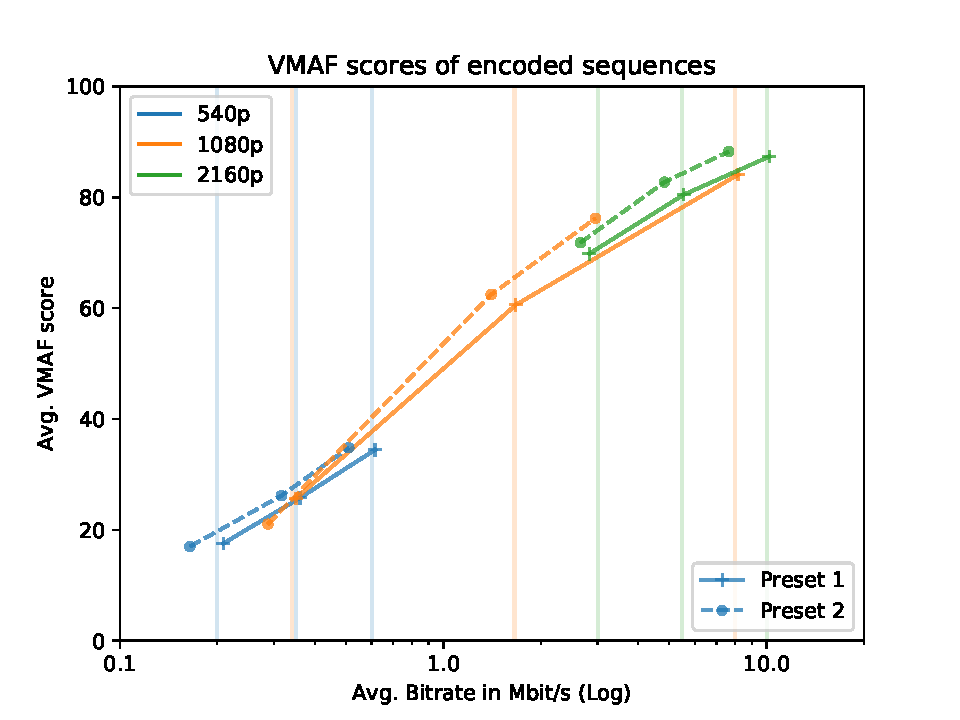
\includegraphics[width=3.5in]{vmaf_final}
	\caption{VMAF scores of encoded videos}
	\label{fig:vmaf:bitrates}
\end{figure}
